\documentclass[a4paper, 11pt]{article}
\usepackage[utf8]{inputenc}
\usepackage[left=2cm, top=3cm, text={17cm, 24cm}]{geometry}
\usepackage[IL2]{fontenc}
\usepackage{times}
\usepackage{caption}
\usepackage[unicode]{hyperref}
\usepackage[ruled, noline, linesnumbered , longend, czech]{algorithm2e}
\usepackage{graphics}
\usepackage{pdfpages}
\usepackage{pdflscape}
\usepackage{graphicx}
\usepackage{multirow}
\usepackage{pict2e}
\usepackage[parfill]{parskip}

\captionsetup[table]{name=Tabulka}
\captionsetup[figure]{name=Obrázek}

\setlength{\parindent}{1pc}

\begin{document}

\begin{titlepage}

    \begin{center}
        \Huge
        \textsc{Vysoké učení technické v Brně\\\huge{Fakulta informačních technologií} }\\
        \vspace{\stretch{0,381966}}
        \LARGE{Typografie a publikování -- 3. projekt\\}
        \Huge{Tabulky a obrázky}
        \vspace{\stretch{0,61034}}
    \end{center}
    \LARGE{3. dubna 2021} 
    \hfill
    \LARGE{Pavel Heřmann}
\end{titlepage}

\section{Úvodní strana}
Název práce umístěte do zlatého řezu a nezapomeňte uvést dnešní datum a vaše jméno a příjmení.



\section{Tabulky}
Pro sázení tabulek můžeme použít buď prostředí \verb=tabbing= nebo prostředí \verb=tabular.=



\subsection{Prostředí \texttt{tabbing}}
Pro použití \texttt{tabbing} vypadá tabulka následovně:
\par

\begin{tabbing}
\hspace{8em}    \= \hspace{3.5em}     \= \hspace{1em} \kill
\textbf{Ovoce}  \>\textbf{Cena}     \>\textbf{Množství} \\
Jablka          \>25,90             \>3 kg \\
Hrušky          \>27,40             \>2,5 kg \\
Vodní melouny   \>35,–              \>1 kus \\
\end{tabbing}
Toto prostředí se dá také použít pro sázení algoritmů, ovšem vhodnější je použití prostředí \verb=algorithm= nebo \verb=algorithm2e= (viz sekce 3).

\subsection{Prostředí \texttt{tabular}}
Další možností, jak vytvořit tabulku, je použití prostředí \texttt{tabular.} Tabulky pak budou vypadat takto\footnote{Kdyby byl problém s \texttt{cline}, zkuste se podívat třeba sem: \hyperlink{http://www.abclinuxu.cz/tex/poradna/show/325037}{http://www.abclinuxu.cz/tex/poradna/show/325037}.}:

\vspace{1em}

\begin{table}[h!]
\catcode`-=12
\label{tabulka1}
    \begin{center}
        \begin{tabular}{|c|c|c|}
            \hline
            & \multicolumn{2}{|c|}{\textbf{Cena}} \\
            \cline{2-3}
            \textbf{Měna} & \textbf{nákup} & \textbf{prodej} \\
            \hline
            EUR & 25.227 & 26.943 \\
            GBP & 29.368 & 31.492 \\
            USD & 21.260 & 22.661 \\
            \hline
        \end{tabular}
    \caption{Tabulka kurzů k dnešnímu dni}
    \end{center}
\end{table}        


\begin{table}[h!]
\label{tabulka2}
    \begin{center}
        \begin{tabular}{|c|c|}
            \hline
            A          & ${\neg{A}}$ \\
            \hline
            \textbf{P} & N        \\
            \hline
            \textbf{O} & O        \\
            \hline
            \textbf{X} & X        \\
            \hline
            \textbf{N} & P       \\
            \hline
        \end{tabular}
        \begin{tabular}{|c|c|c|c|c|c|}
            \hline
            \multicolumn{2}{|c|}{\multirow{2}{*}{A ${\wedge}$ B}} & \multicolumn{4}{c|}{B} \\ \cline{3-6} 
            \multicolumn{2}{|c|}{}  & \textbf{P}    &\textbf{O}   &\textbf{X}   &\textbf{N} \\ 
            \hline
            \multirow{4}{*}{A}  &\textbf{P}     & P    & O   & X   & N   \\ \cline{2-6} 
                                &\textbf{P}     & O    & O   & N   & N   \\ \cline{2-6} 
                                &\textbf{P}     & X    & N   & X   & N   \\ \cline{2-6} 
                                &\textbf{P}     & N    & N   & N   & N   \\ \hline
        \end{tabular}
        \begin{tabular}{|c|c|c|c|c|c|}
            \hline
            \multicolumn{2}{|c|}{\multirow{2}{*}{A ${\lor}$ B}} & \multicolumn{4}{c|}{B} \\ \cline{3-6} 
            \multicolumn{2}{|c|}{}  & \textbf{P}    &\textbf{O}   &\textbf{X}   &\textbf{N} \\ 
            \hline
            \multirow{4}{*}{A}  &\textbf{P}     & P    & O   & X   & N   \\ \cline{2-6} 
                                &\textbf{P}     & O    & O   & N   & N   \\ \cline{2-6} 
                                &\textbf{P}     & X    & N   & X   & N   \\ \cline{2-6} 
                                &\textbf{P}     & N    & N   & N   & N   \\ \hline
        \end{tabular}
        \begin{tabular}{|c|c|c|c|c|c|}
            \hline
            \multicolumn{2}{|c|}{\multirow{2}{*}{A ${\to}$ B}} & \multicolumn{4}{c|}{B} \\ \cline{3-6} 
            \multicolumn{2}{|c|}{}  & \textbf{P}    &\textbf{O}   &\textbf{X}   &\textbf{N} \\ 
            \hline
            \multirow{4}{*}{A}  &\textbf{P}     & P    & O   & X   & N   \\ \cline{2-6} 
                                &\textbf{P}     & O    & O   & N   & N   \\ \cline{2-6} 
                                &\textbf{P}     & X    & N   & X   & N   \\ \cline{2-6} 
                                &\textbf{P}     & N    & N   & N   & N   \\ \hline
        \end{tabular}
    \caption{Protože Kleeneho trojhodnotová logika už je ,,zastaralá", uvádíme si zde příklad čtyřhodnotové logiky}
    \end{center}
\end{table}
%POSUNOUT FOOTNOTE NAHORU



\newpage
\section{Algoritmy}
    Pokud budeme chtít vysázet algoritmus, můžeme použít prostředí \texttt{algorithm}\footnote{Pro nápovědu, jak zacházet s prostředím \texttt{algorithm}, můžeme zkusit tuhle stránku: \newline \hyperlink{http://ftp.cstug.cz/pub/tex/CTAN/macros/latex/contrib/algorithms/algorithms.pdf}{http://ftp.cstug.cz/pub/tex/CTAN/macros/latex/contrib/algorithms/algorithms.pdf}.}nebo \texttt{algorithm2e}\footnote{Pro \texttt{algorithm2e} zase tuhle:
    \hyperlink{http://ftp.cstug.cz/pub/tex/CTAN/macros/latex/contrib/algorithm2e/doc/algorithm2e.pdf}{http://ftp.cstug.cz/pub/tex/CTAN/macros/latex/contrib/algorithm2e/doc/algorithm2e.pdf}}.
    Příklad použití prostředí \texttt{algorithm2e} viz Algoritmus 1.
    
    \vspace{2em}

\begin{algorithm}[H]
    \label{algoritmus}
    \SetNlSty{}{}{:}
    \SetInd{1em}{1em}
    \KwIn{$(X_{t - 1}, u_t, z_t)$}
    \KwOut{$X_t$}
    \BlankLine
    $ \overline{X_t} = X_t = 0 $ \\
    \For{$k = 1 \textrm{\emph{ to }}M$}
    { 
    $x_t^{[k]} = sample\_motion\_model(ut,x{t-1}^{[k]})$ \\
    $\omega_t^{[k]} = measurement\_model(zt,x{t}^{[k],m_{t-1}})$ \\
    $m_t^{[k]} =updated\_occupancy\_grid(zt,x{t}^{[k]},m_{t-1}^{[k]})$ \\
    $\overline{X_t} = \overline{X_t} + \langle x_x^{[m]}, \omega_t^{[m]} \rangle$ \\
    }
    \For{$k = 1 \textrm{\emph{ to }}M$}
    {
        draw $i$ with probability $ \approx\omega_t^{[i]}$ \\
        add $\langle x_x^{[k]}, m_t^{[k]} \rangle\textrm{ to }X_t$ \\
    }
    \Return{$X_t$}
    \caption{FastSLAM}
\end{algorithm}
\hspace{4em}


\section{Obrázky}

Do našich článků můžeme samozřejmě vkládat obrázky. Pokud je obrázkem fotografie, můžeme klidně
použít bitmapový soubor. Pokud by to ale mělo být nějaké schéma nebo něco podobného, je dobrým
zvykem takovýto obrázek vytvořit vektorově.

\begin{figure}[h!]
\label{obr1}
    \centering
    \scalebox{0.40}{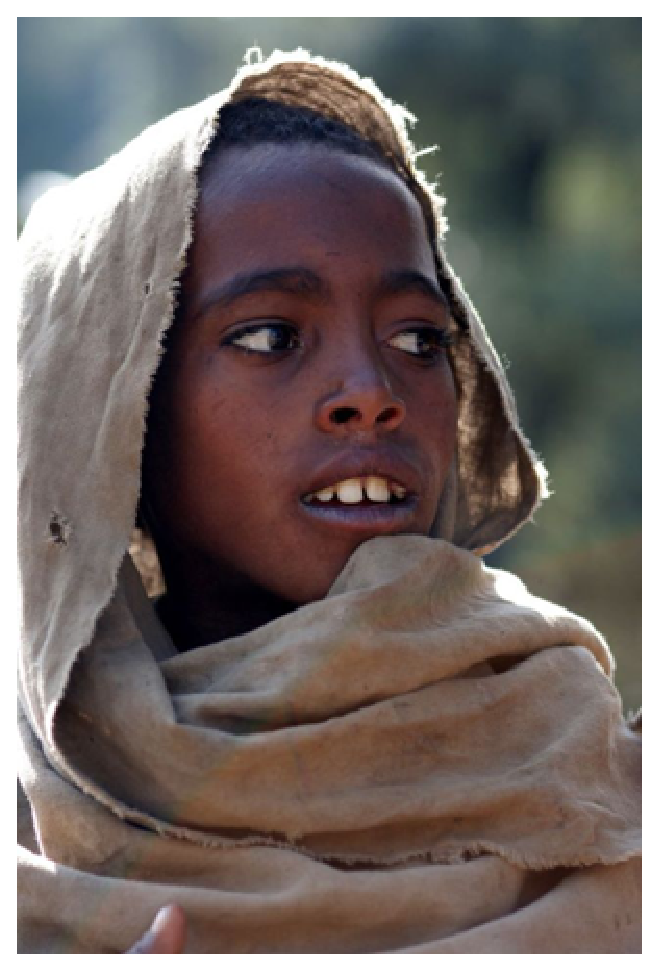
\includegraphics{etiopan.eps}}
    \scalebox{0.40}{\reflectbox{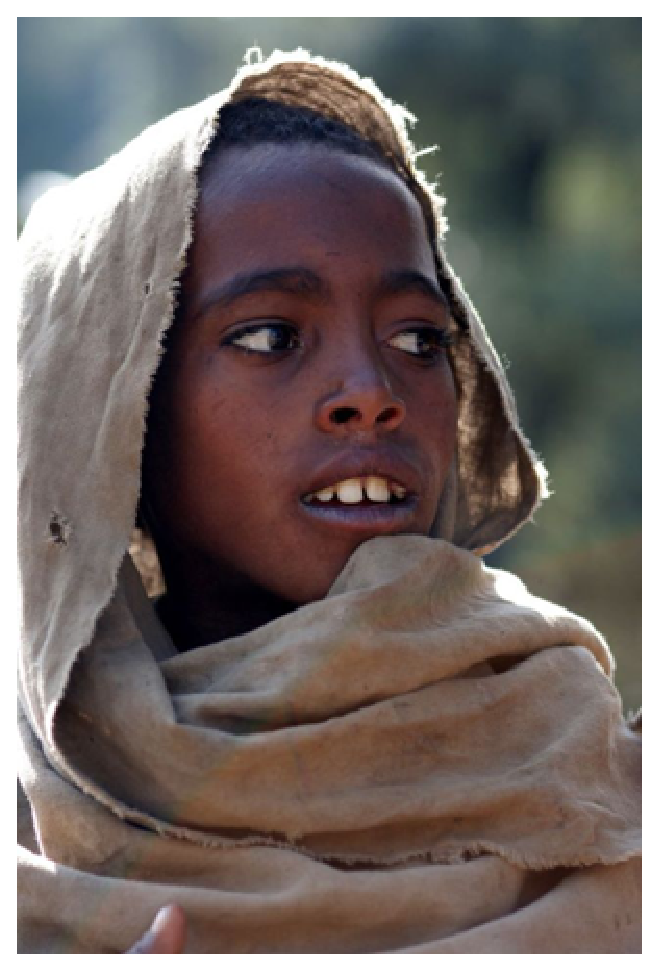
\includegraphics{etiopan.eps}}}
    \caption{Malý Etiopánek a jeho bratříček}
    \label{fig:my_label}
\end{figure}
\newpage

Rozdíl mezi vektorovým \dots 
\par

\begin{figure}[h!]
\label{obr2}
    \centering
    \scalebox{0.45}{
\includegraphics{oniisan.eps}}
    \caption{Vektorový obrázek}
    \label{fig:my_label}
\end{figure}

\dots a bitmapovým obrázkem
\par
\begin{figure}[h!]
\label{obr3}
    \centering
    \scalebox{0.68}{
\includegraphics{oniisan2.eps}}
    \caption{Bitmapový obrázek}
    \label{fig:my_label}
\end{figure}
\vspace{2em}
se projeví například při zvětšení.
\par
Odkazy (nejen ty) na obrázky \hyperref[obr1]{1}, \hyperref[obr2]{2} a \hyperref[obr3]{3}, na tabulky \hyperref[tabulka1]{1} a \hyperref[tabulka2]{2} a také na algoritmus \ref{algoritmus} jsou udělány pomocí křižových odkazů. Pak je ovšem potřeba zdrojový soubor přeložit dvakrát.
\par
Vektorové obrázky lze vytvořit i přímo v \LaTeX u, například pomocí prostředí \texttt{picture}.

\begin{landscape}
    \setlength{\unitlength}{2em}
    \thicklines
    \begin{picture}(10,11)
    %kostra domu
    \put(0,-10){\line(0,1){18}}
    \put(0,8){\line(1,0){20}}
    \put(0,-10){\line(1,0){30}}
    \put(20,-10){\line(0,1){18}}
    %garaz
    \put(30,-10){\line(0,1){9}}
    \put(20,-1){\line(1,0){10}}
    \put(21,-10){\line(0,1){8}}
    \put(29,-10){\line(0,1){8}}
    \put(21,-2){\line(1,0){8}}
    %dvere
    \put(8,-10){\line(0,1){5}}
    \put(12,-10){\line(0,1){5}}
    \put(8,-5){\line(1,0){4}}
    \put(9,-8){\circle*{0.5}}
    %okno vlevo dole
    \put(2,-7){\line(1,0){4}}
    \put(2,-7){\line(0,1){4}}
    \put(2,-3){\line(1,0){4}}
    \put(6,-7){\line(0,1){4}}
    %okno vpravo dole
    \put(14,-7){\line(0,1){4}}
    \put(18,-7){\line(0,1){4}}
    \put(14,-7){\line(1,0){4}}
    \put(14,-3){\line(1,0){4}}
    %okno vpravo nahore
    \put(14,1){\line(0,1){4}}
    \put(18,1){\line(0,1){4}}
    \put(14,1){\line(1,0){4}}
    \put(14,5){\line(1,0){4}}
    %okno vlevo nahore
    \put(2,1){\line(1,0){4}}
    \put(2,1){\line(0,1){4}}
    \put(2,5){\line(1,0){4}}
    \put(6,1){\line(0,1){4}}
    %slunce
    \put(28, 9){\circle*{6}}
    
    
    \end{picture}
\end{landscape}


\end{document}

